\documentclass[a4paper, 12pt]{article}

%\usepackage{cmap}
\usepackage[T2A]{fontenc}
\usepackage[utf8]{inputenc}
\usepackage[english, russian]{babel}
\usepackage{graphicx}
\usepackage[top=1in, bottom=1in, left=3.2cm, right=2.6cm]{geometry}
\graphicspath{./}
\usepackage{biblatex}
\addbibresource{lib.bib}
\linespread{1.5}
\usepackage{ragged2e}
\justifying
\usepackage{listings}
\usepackage{color}


\begin{document}
	
\begin{titlepage}
	\fontsize{12pt}{12pt}\selectfont
	\begin{figure}[t!]
		\centering
		
\includegraphics[scale=0.8]{bmstu}
	\end{figure}
	
	\noindent\rule{15cm}{3pt}
	\newline\newline
	\noindent 
	ФАКУЛЬТЕТ 
	\underline{«Информатика и системы управления»} \newline\newline
	
	\noindent КАФЕДРА \underline{«Программное обеспечение ЭВМ и информационные технологии»}\newline\newline\newline\newline\newline
	
	\centering {\Large Отчет по лабораторной работе № 4}
	\vspace{4mm}
	
	\centering {\Large По курсу: "Функциональное и логическое программирование"
		\vspace{8mm}	
		
		}
	\vspace{8mm}
	
	
	\begin{flushright}
		{\small	Студент:\\ Турсунов Жасурбек Рустамович \\ Группа: ИУ7-66Б
			\vspace{3mm}
			\\Преподователи: \\ Толпинская Наталья Борисовна \\ Строганов Юрий Владимирович}
	\end{flushright}
	
	\begin{center}
		\vfill
		Москва, \the\year
		~г.
	\end{center}
\end{titlepage}

\tableofcontents
\clearpage
\newpage

\textbf{Цель работы:} приобрести навыки работы с управляющими структурами Lisp.
\\ \hspace*{5mm} \textbf{Задачи работы:} изучить работу функций с произвольным количеством аргументов, функций разрушающих и неразрушающих структуру исходных аргументов.


\section*{Введение}
\addcontentsline{toc}{section}{Введение}

\hspace*{5mm} Многие стандартные функции Lisp являются формами и реализуют особый способ работы со своими аргументами. К таким функциям относятся функции, позволяющие работать с произвольным количеством аргументов: and, or, append, или особым образом обрабатывающее свои аргументы: функции cond, if, append, remove, reverse, substitute.
\\ \hspace*{5mm} Если на вход функции подается структура данных(списков), то возникает вопрос: сохранится ли возможность в дальнейшем работать с исходными струтурами, или они изменятся в процессе реализации функции. В Lisp существуют функции, использующие списки в качестве аргументов и разрушающие структуру исходных аргументов при этом часть из них позволяет использовать произвольное количество аргументов, а часть нет.
\clearpage
\newpage


\definecolor{codegreen}{rgb}{0,0.6,0}
\definecolor{codegray}{rgb}{0.5,0.5,0.5}
\definecolor{codepurple}{rgb}{0.58,0,0.82}
\definecolor{backcolour}{rgb}{0.95,0.95,0.92}

\lstdefinestyle{mystyle}{
	backgroundcolor=\color{backcolour},   
	commentstyle=\color{codegreen},
	keywordstyle=\color{magenta},
	numberstyle=\tiny\color{codegray},
	stringstyle=\color{codepurple},
	basicstyle=\ttfamily\footnotesize,
	breakatwhitespace=false,         
	breaklines=false,                 
	captionpos=b,                    
	keepspaces=true,                 
	numbers=left,                    
	numbersep=5pt,                  
	showspaces=false,                
	showstringspaces=false,
	showtabs=false,                  
	tabsize=4
}

\lstset{style=mystyle}

\section*{Задание 7}
\addcontentsline{toc}{section}{Задание 7}
Написать функцию, которая переводит температуру в системе Фаренгейта температуру по Цельсию (defun f-to-c (temp)...):\\
\begin{lstlisting}
	(defun f-to-c (temp)
		(* (- temp 32.0) 5/9)
	)
\end{lstlisting}

Как бы назывался роман Р.Брэдбери "+451 по Фаренгейту" в системе по Цельсию:
\\
\begin{lstlisting}
	>(f-to-c 451)
	;232.77779
\end{lstlisting}


\section*{Задание 8}
\addcontentsline{toc}{section}{Задание 8}
Что получится при вычисления каждого из выражений?\\
\hspace*{20mm}\begin{tabular}{ | l | l | }
	\hline
	\textbf{Выражение} & \textbf{Результат} \\ \hline
	(list 'cons t Nil) & (CONS T NIL) \\ \hline
	(eval(list 'cons t Nil)) & T \\ \hline
	(eval(eval(list 'cons t Nil))) & Undefined function T \\ \hline
	(eval Nil) & NIL \\ \hline
	(list 'eval Nil) & (EVAL NIL) \\ \hline
	(eval(list 'eval Nil)) & NIL \\ \hline
	(apply \#cons "(t nil)) & bad syntax for complex number: \#CONS \\ \hline
\end{tabular}



\section*{Дополнительно 1}
\addcontentsline{toc}{section}{Дополнительно 1}
Написать функцию, вычисляющую катет по заданной гипотенузе и другому катету прямоугольного треугольника, и составить диаграмму ее вычисления.
\begin{lstlisting}
		(defun kateta(a b)
			(sqrt (-(* a a) (* b b)))
		)
		
		>(kateta 5 4)
		;3
\end{lstlisting}
\begin{figure}[h!]
	\centering 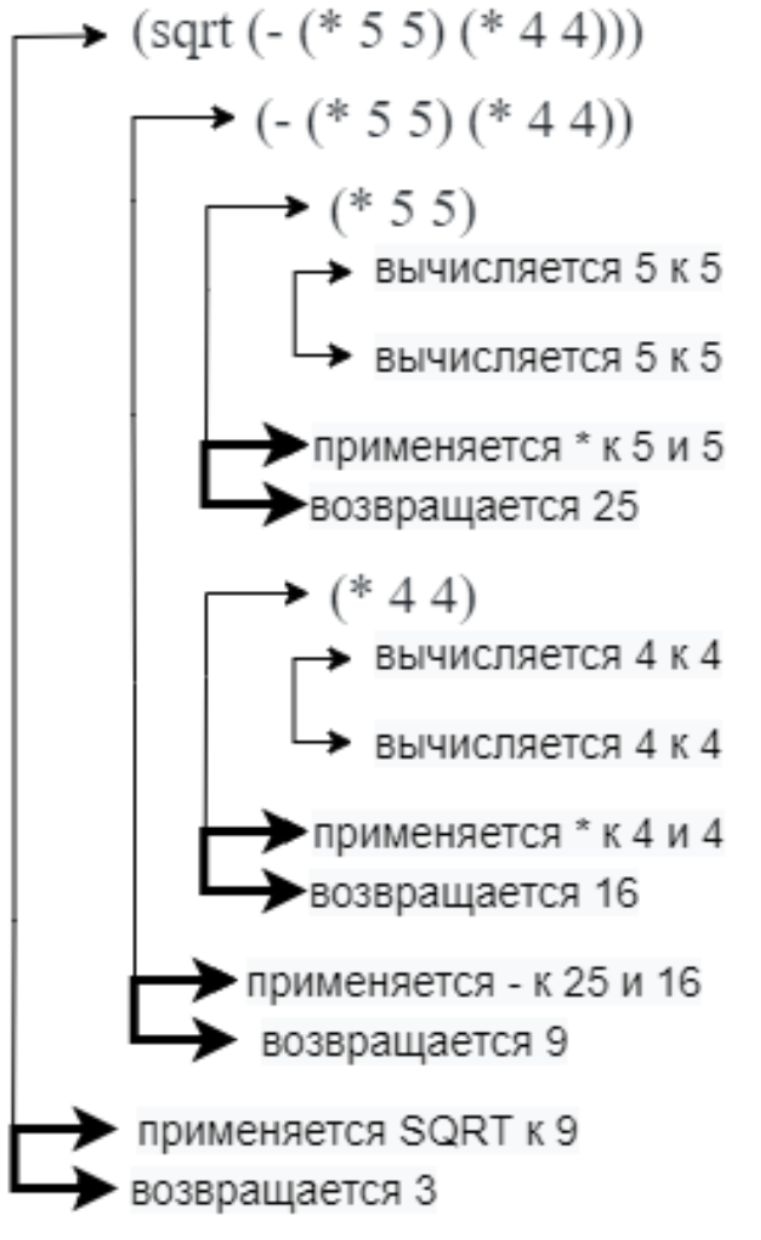
\includegraphics[scale=0.8]{dop1}
	\centering\caption{диаграмма функции вычисляющую катет}
\end{figure}

\section*{Дополнительно 2}
\addcontentsline{toc}{section}{Дополнительно 2}
Написать функцию, вычисляющую площадь трапеции по ее основаниям и высоте, и составить диаграмму ее вычисления\\ \\
\begin{lstlisting}
	(defun area(a b h)
		(* (+ a b) h 0.5)
	)
	
	>(area 3 4 5)
	;17.5
\end{lstlisting}
\begin{figure}[h!]
	\centering 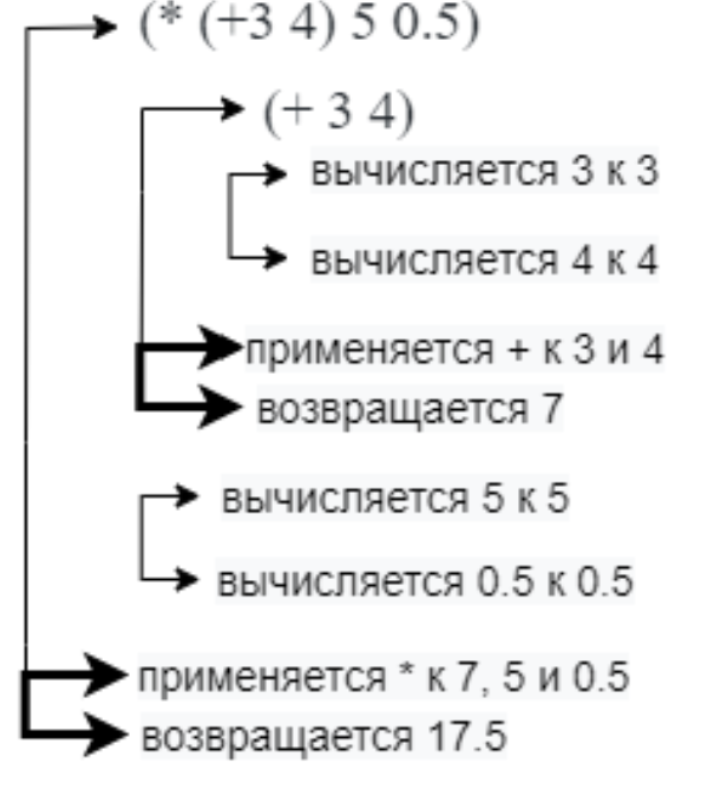
\includegraphics[scale=0.8]{dop2}
	\centering\caption{диаграмма функции вычисляющую площадь трапеции}
\end{figure}

\section*{Ответы на вопросы:}
\addcontentsline{toc}{section}{Ответы на вопросы}
\hspace*{-7mm} \textbf{1) Трактовка элементов списка:}

\hspace*{-6mm}Списки представлены с помощью списковых ячеек. Списочная ячейка состоит из двух частей, полей car и cdr. Каждое из полей содержит указатель. Указатель может ссылаться на другую списочную ячейку или на некоторый другой Lisp объект, как, например, атом.
\\ Указатели между ячейками образуют цепочку, по которой можно из предыдущей ячейки попасть в следующую и так, наконец, до атомарных объектов. Каждый известный системе атом записан в определённом месте памяти лишь один раз.
\\Если это  не стоит блокировка вычисления(quote, '), то первый элемент трактуется как имя функции, остальные — как аргументы.

\hspace*{-13mm} \textbf{2) Порядок реализации программы:}
\\ Реализации программы определяется базовой функцией eval:
\clearpage
\newpage
\begin{figure}[h!]
	\centering 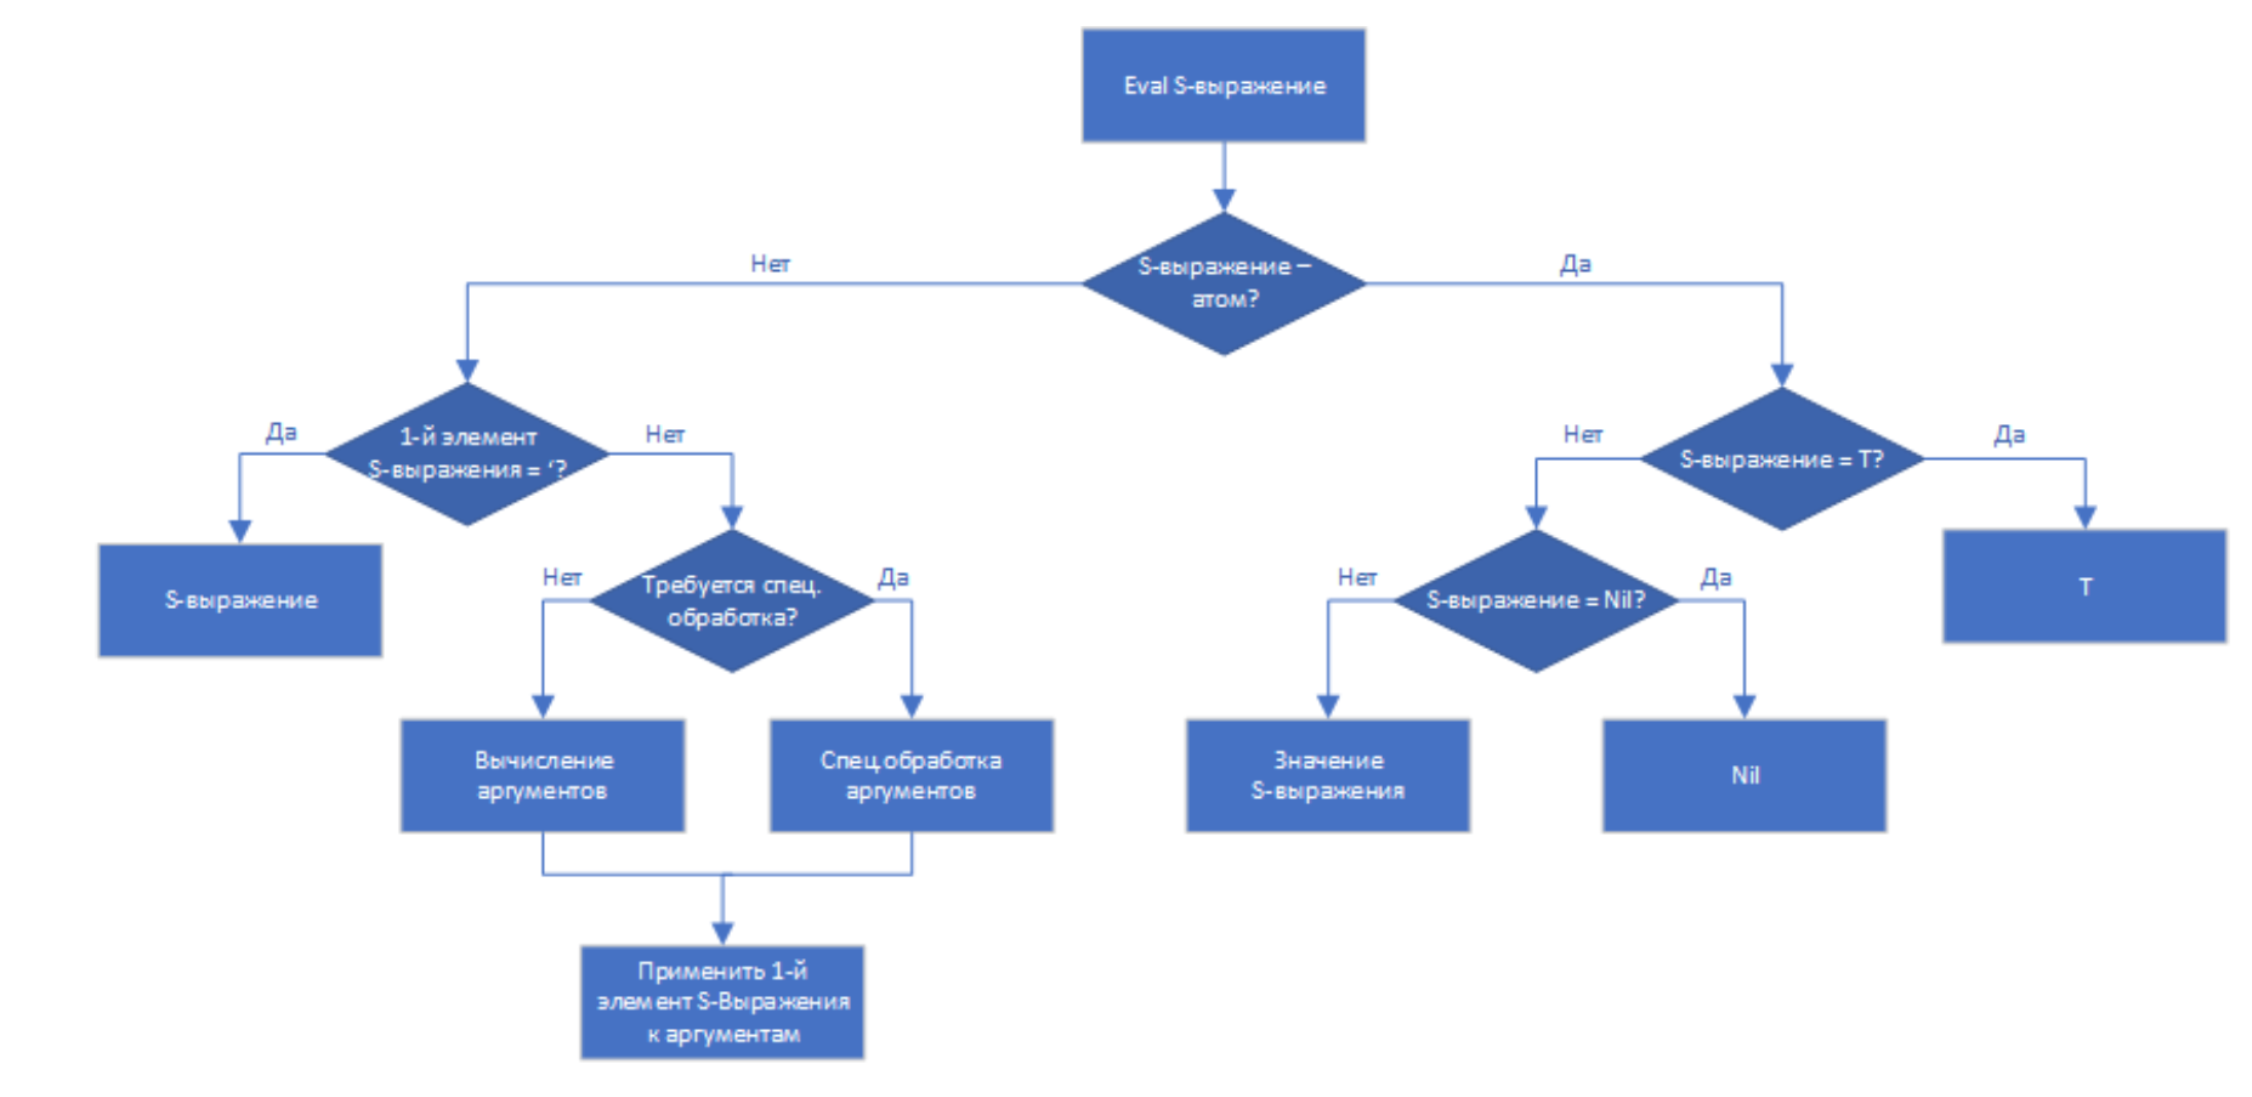
\includegraphics[scale=0.7]{eval}
\end{figure}
\hspace*{-8mm} \textbf{3) Способы определения функций}
\\Новые функции можно определить с помощью оператора defun. Он принимает три или более аргументов: имя, список параметров и ноль или более выражений, которые составляют тело функции. 

(defun func\_name (arg1 arg2 ... argN) func\_body)

Но функция не обязательно должна иметь имя, для того, чтобы определить функцию, не имеющую имени, необходимо воспользоваться лямбда-выражением. Лямбда-выражение – это список, содержащий символ lambda и следующие за ним список аргументов и тело, состоящее из нуля или более выражений.

(lambda (arg1 arg2 .. argN) func\_body)

\hspace*{-8mm} \textbf{4) Синтаксическая форма и хранение программы в памяти}
\\

\end{document}